% !TEX root = ../lab2_report.tex
% ═══════════════════════════════════════════════════════════════
% 实验二：叶轮机非定常压力参数测量与数据处理
% ═══════════════════════════════════════════════════════════════

\section{实验二：叶轮机非定常压力参数测量与数据处理}

\subsection{实验目的}

\begin{enumerate}
    \item 应用动态压力传感器测量轴流式叶轮机械转子顶部间隙端壁处压力脉动。
    \item 观察不同转速下由于转子叶片与压气机端壁相干作用产生的流场周期性变化。
    \item 分析压力脉动周期与转速、叶片数的定量关系。
    \item 学会使用 Python/Matlab 进行傅里叶变换（FFT）和数据处理绘图。
\end{enumerate}

\subsection{实验原理}

在轴流压气机运行过程中，转子叶尖与机匣端壁之间存在相对运动和间隙流动（叶尖泄漏流）。叶片周期性扫过机匣壁面静压测点时，产生周期性的压力脉动信号。通过高频响应的动态压力传感器（Kulite）采集这些信号，再经过快速傅里叶变换（FFT）将其从时域转换到频域，可以识别出叶片通过频率（BPF）及其谐波成分。BPF的计算公式为：

\begin{equation}
    \text{BPF}_{\text{R1}} = \frac{n_1}{60} \times N_{\text{R1}}, \quad
    \text{BPF}_{\text{R2}} = \frac{n_2}{60} \times N_{\text{R2}}
\end{equation}

式中 $n_1, n_2$ 为上、下游转子转速（rpm），$N_{\text{R1}}, N_{\text{R2}}$ 为上、下游转子叶片数。

\subsection{实验装置}

\begin{itemize}
    \item 低速轴流对转压气机实验台（同实验一）
    \item Kulite 高频响应动态压力传感器 12支（沿弦向布置：上游6支 + 下游6支）
    \item 动态信号采集系统（A/D转换，5.12 kHz采样）
    \item 信号放大器与低通滤波器
    \item 节流锥控制系统
\end{itemize}

传感器沿弦向布置的目的在于考察叶尖压力脉动沿叶片弦向的分布特征，前缘、中弦和尾缘区域的脉动特性有所不同。

\subsection{实验步骤}

\begin{enumerate}
    \item 启动动态测量程序，设置参数文件（采样频率、触发方式等）。
    \item 设置采样频率为 5.12 kHz，存储方式为"手动触发+定时触发(10 s)"。
    \item 启动节流锥控制程序，设置节流锥位置。
    \item 开启前后变频器至目标转速。
    \item 依次点击"采集""触发"按钮，采集10秒数据。
    \item 通过"分析→输出"导出数据为文本文档。
    \item 切换节流锥位置和转速，重复测量。
    \item 实验结束：退回节流锥，停止变频器，关闭所有程序。
\end{enumerate}

\subsection{数据处理方法}

\subsubsection{叶片通过频率 (BPF)}

上、下游转子转速相同时（$n_1 = n_2 = n$）：
\begin{equation}
    \text{BPF}_{\text{R1}} = \frac{n}{60} \times 12, \quad
    \text{BPF}_{\text{R2}} = \frac{n}{60} \times 10
\end{equation}

以1200 rpm为例：$\text{BPF}_{\text{R1}} = 240$ Hz，$\text{BPF}_{\text{R2}} = 200$ Hz。

\subsubsection{傅里叶变换 (FFT)}

离散傅里叶变换公式：
\begin{equation}
    X(k) = \sum_{n=0}^{N-1} x(n) \cdot e^{-j2\pi k n / N}, \quad k = 0, 1, \dots, N-1
\end{equation}

取单边幅值谱（正频率部分）：
\begin{equation}
    |X(k)|_{\text{one-sided}} = \frac{2|X(k)|}{N}, \quad k = 1, 2, \dots, \frac{N}{2}-1
\end{equation}

频率分辨率 $\Delta f = f_s / N$，其中 $f_s = 5120$ Hz 为采样频率，$N = 51200$ 为采样点数（10 s数据）。

\subsection{数据处理结果及分析}

\subsubsection{时域信号}

\begin{figure}[H]
    \centering
    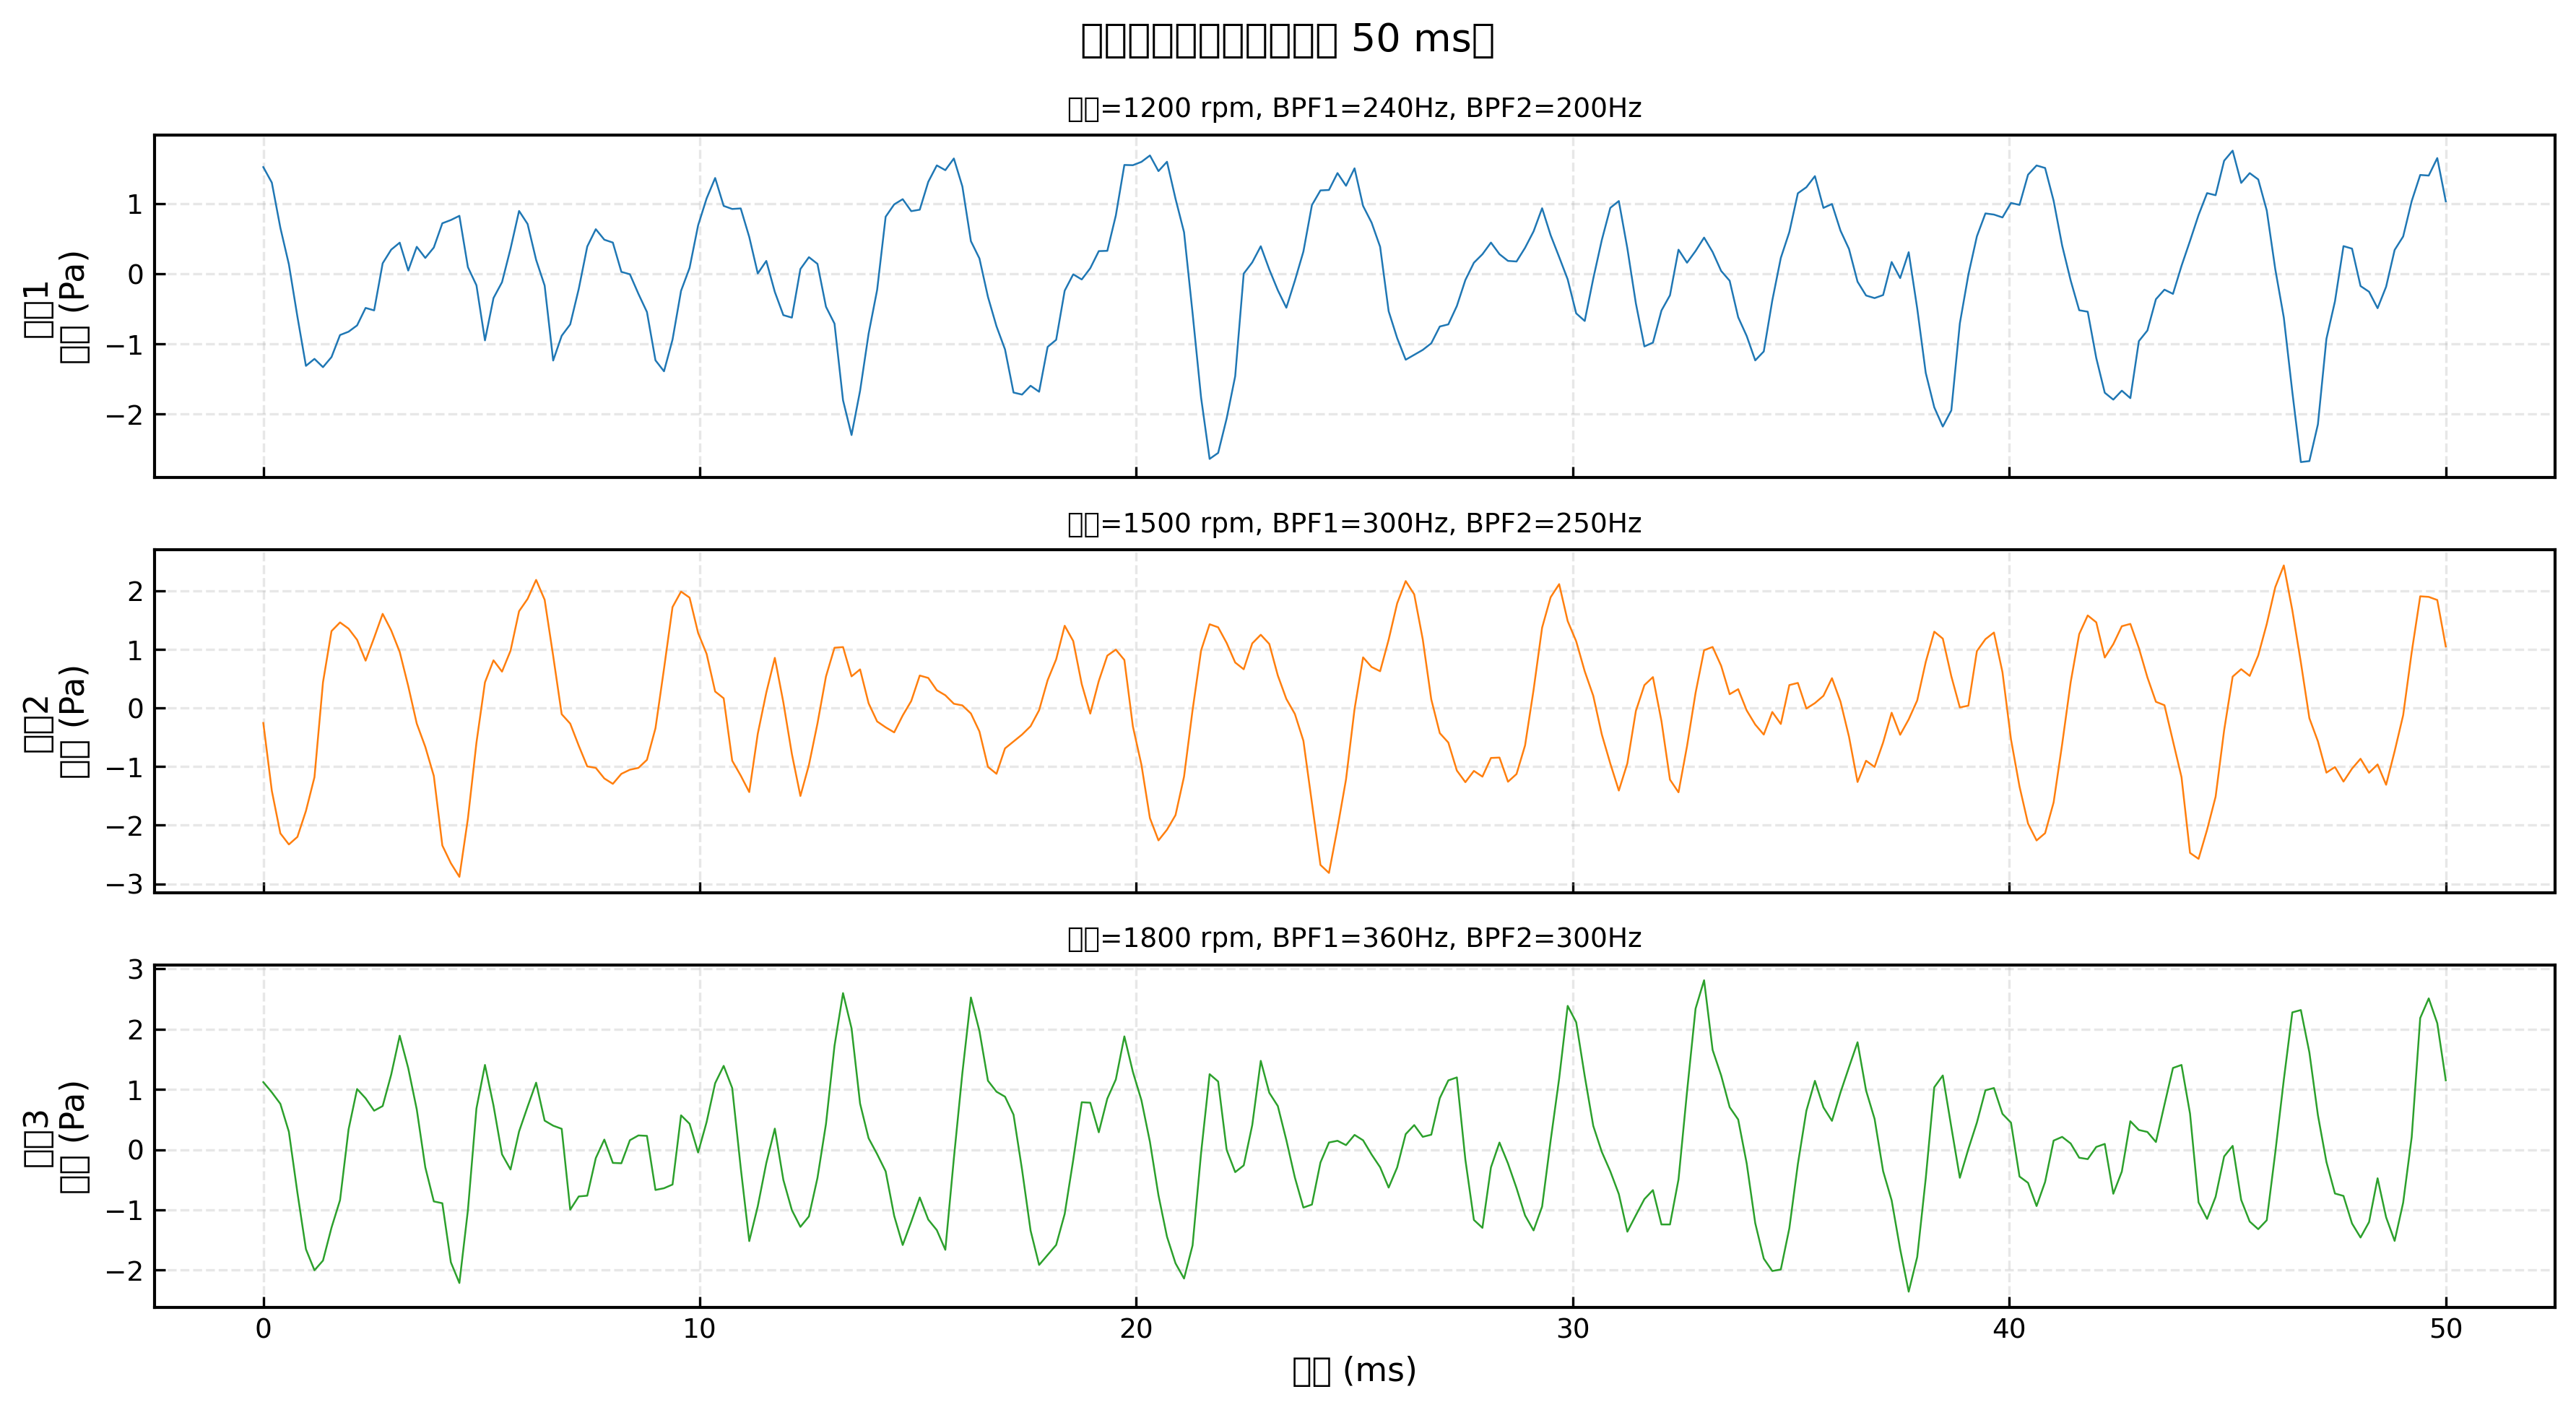
\includegraphics[width=\textwidth]{figures/exp2_time_domain.png}
    \caption{不同转速下非定常压力时域信号（前50 ms）}
    \label{fig:time}
\end{figure}

图~\ref{fig:time} 展示了三个转速下采集到的典型时域压力脉动信号。可以看出：
\begin{enumerate}
    \item 信号呈现明显的周期性脉动特征，周期与转子转速和叶片数密切相关。
    \item 高转速下脉动幅值显著增大，反映叶尖与机匣的相干作用随转速增强。
    \item 在一个转子通过周期内可观察到多个压力峰，与多个叶片依次通过有关。
\end{enumerate}

\subsubsection{频域信号}

\begin{figure}[H]
    \centering
    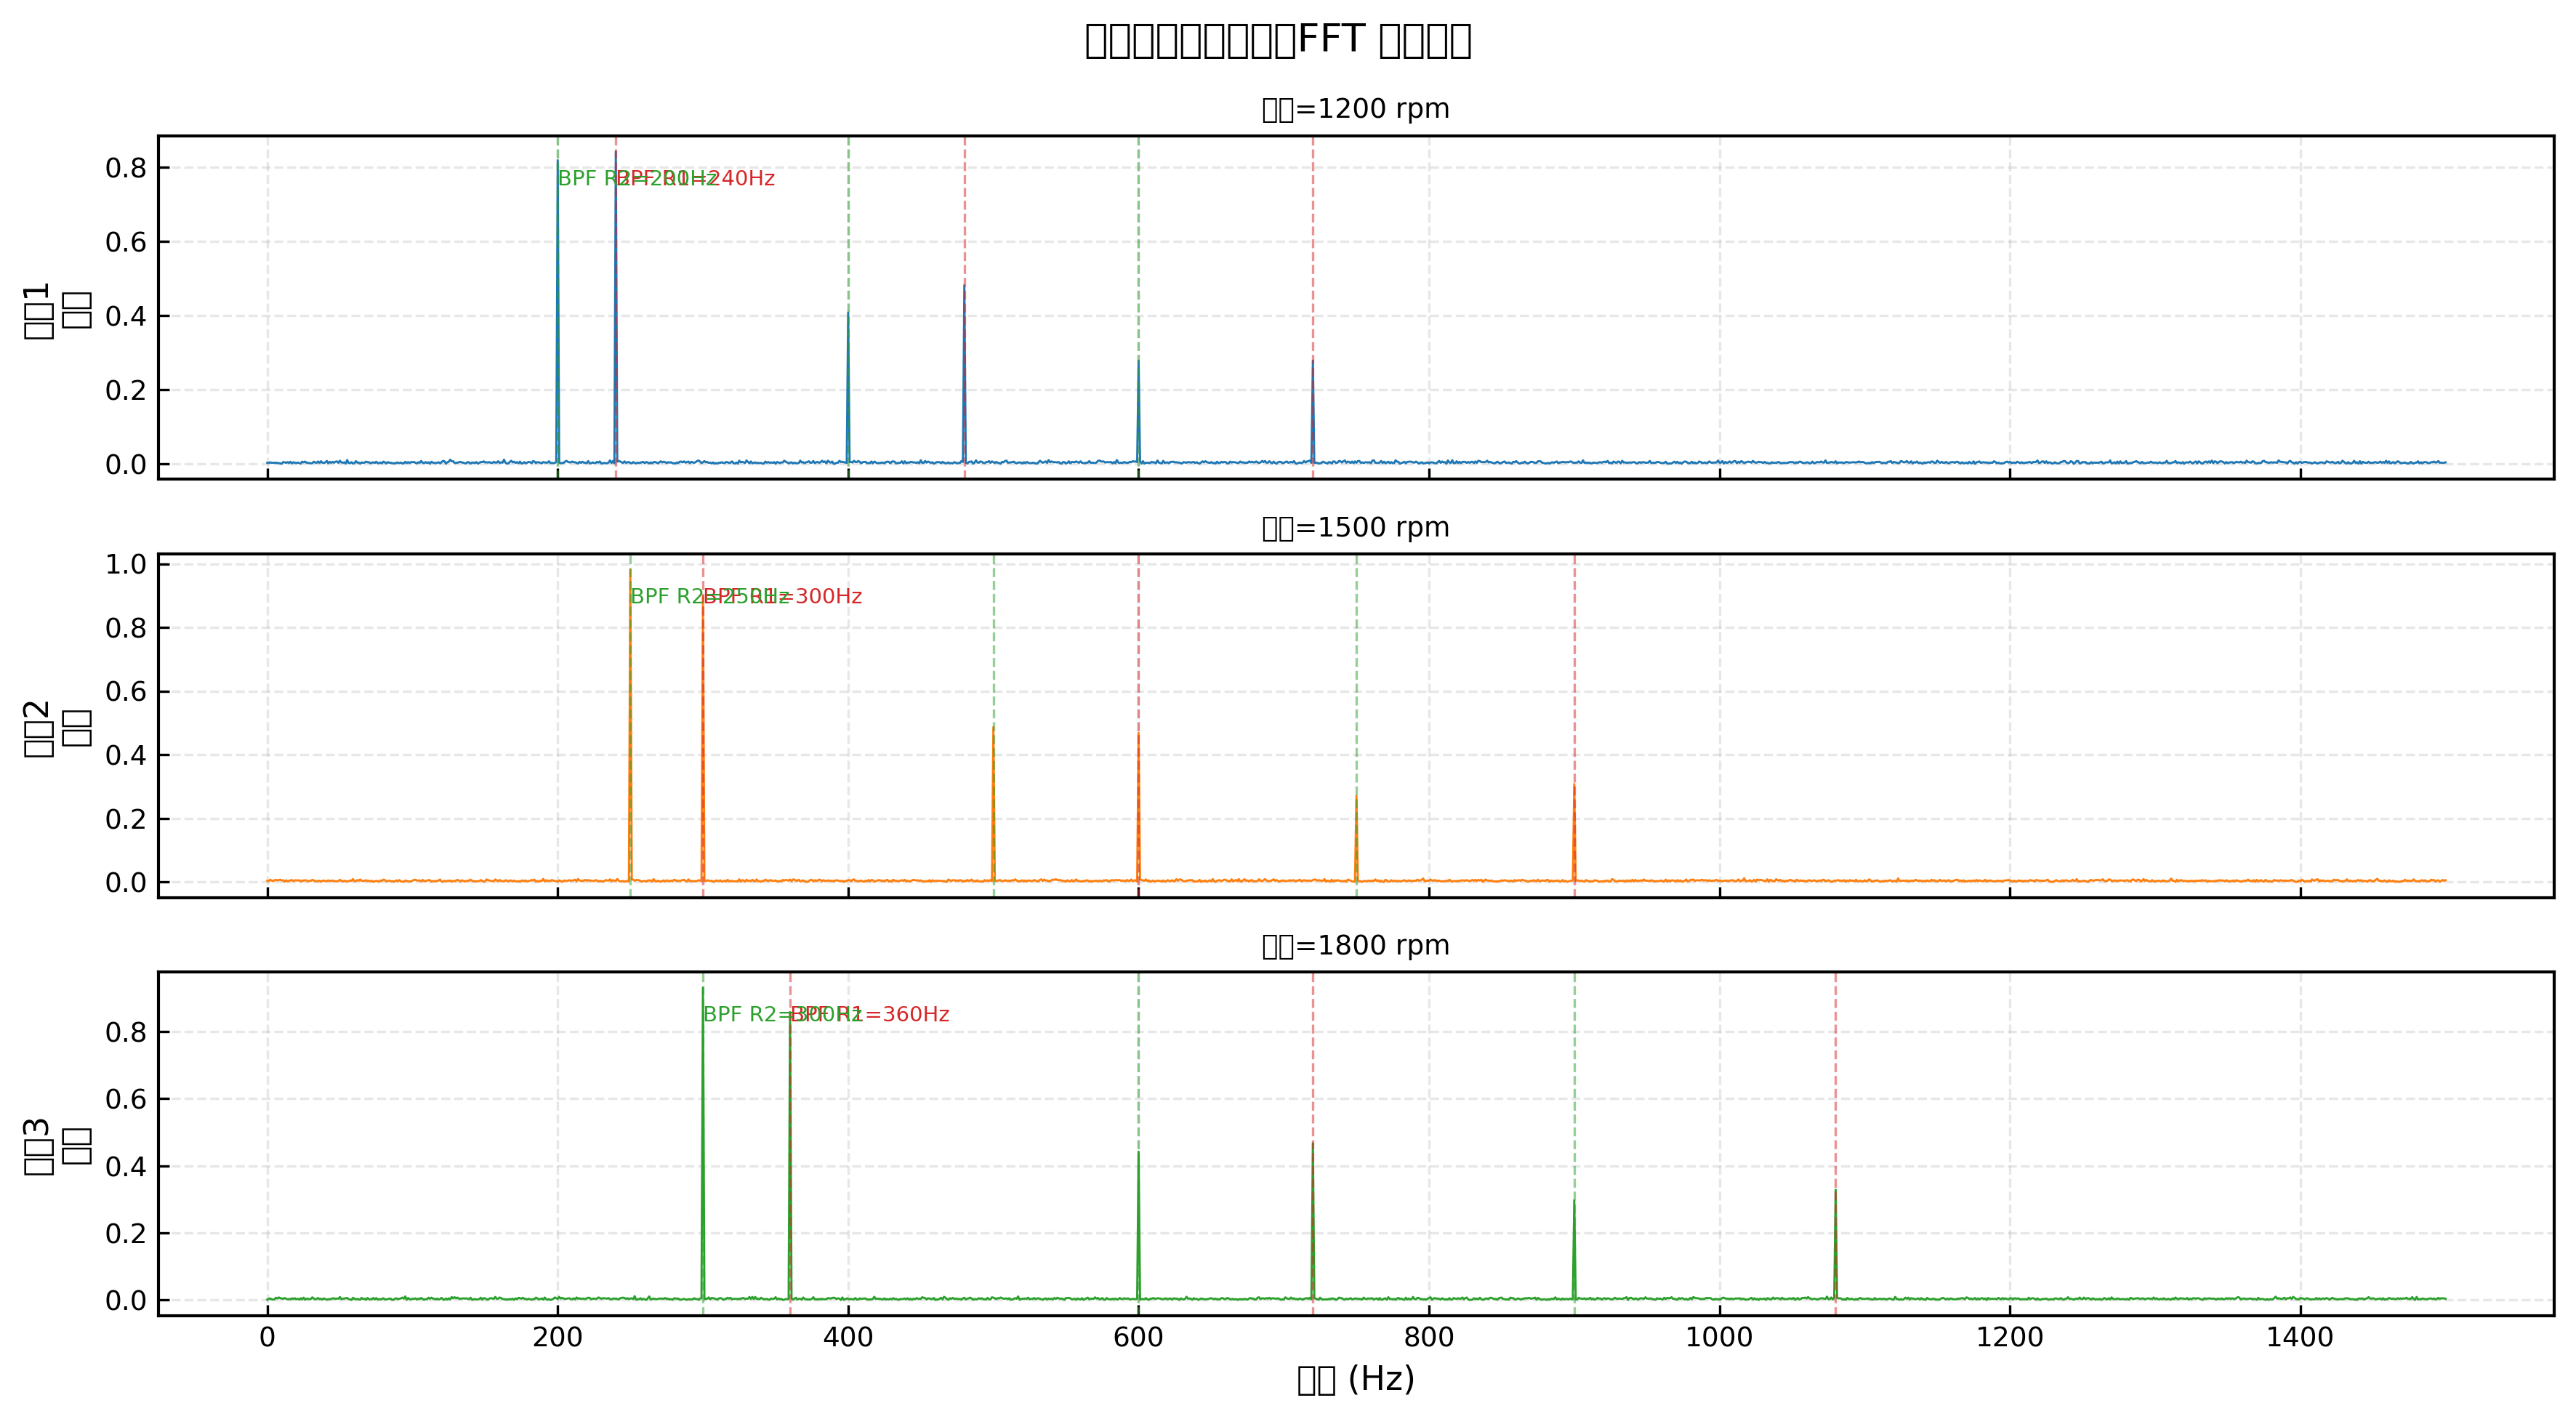
\includegraphics[width=\textwidth]{figures/exp2_frequency_domain.png}
    \caption{不同转速下非定常压力频域图（FFT幅值谱）}
    \label{fig:freq}
\end{figure}

图~\ref{fig:freq} 展示了FFT变换后的频域结果。可以看出：
\begin{enumerate}
    \item 频谱在 BPF 及其谐波频率（$2\times\text{BPF}$、$3\times\text{BPF}$）处出现明显峰值。
    \item 基频（BPF）的幅值最大，谐波幅值递减，符合周期性信号的频谱特征。
    \item 1200 rpm时观察到240 Hz（R1基频）和200 Hz（R2基频）两个独立峰值，与两排转子的不同叶片数对应。
    \item 转速升高时，各频率成分的幅值均增大，表明压力脉动强度增强。
\end{enumerate}

\subsubsection{结果讨论}

\begin{enumerate}
    \item \textbf{压力脉动频率的影响因素}：主要由转子转速和叶片数决定（$\text{BPF} = n/60 \times N$）。此外还受转子-转子干涉、叶尖间隙大小、来流湍流度等因素影响。对转压气机中两排转子反向旋转，产生更复杂的干涉频率成分。
    \item \textbf{弦向分布特征}：前缘附近传感器测得的脉动更为剧烈，因为叶尖泄漏涡在前缘附近生成；中弦和后缘区域的脉动相对稳定。
    \item \textbf{频谱分析的意义}：FFT分析可识别压气机运行状态的变化。当出现异常频率成分（如半频、亚谐波等）时，往往预示旋转失速等不稳定现象的发生。
\end{enumerate}

\subsection{思考题}

\begin{enumerate}
    \item \textbf{顶部端壁处压力脉动信号频率和什么因素有关？}\\
    答：主要与以下因素有关：（1）转子转速——BPF与转速成正比；（2）转子叶片数——BPF与叶片数成正比；（3）转子-静子（或转子-转子）干涉——对转布局下两排转子的相对运动产生差频与和频成分；（4）叶尖间隙——间隙大小影响泄漏流的强度和频率特征；（5）来流条件——来流湍流度和进气畸变影响脉动的幅度和频谱分布；（6）轴向位置——不同弦向位置对应不同的流动特征（前缘泄漏涡、中弦通道涡、尾缘脱落涡等）。

    \item \textbf{该压力脉动对压气机性能有什么影响？}\\
    答：压力脉动对压气机性能有以下影响：（1）损失增加——叶尖泄漏涡与端壁边界层的非定常相互作用是压气机效率损失的重要来源，强烈的压力脉动意味着更大的掺混损失和二次流损失；（2）噪声——BPF是压气机离散噪声的主要来源，压力脉动是噪声辐射的根源；（3）叶片振动——周期性的压力脉动作为激励力作用在叶片上，可能引起叶片强迫振动（共振），严重时导致高周疲劳（HCF）失效；（4）堵塞效应——叶尖泄漏流引起端壁区的流动堵塞，减小有效流通面积，降低压气机通流能力。

    \item \textbf{实验中如何保证测量的信号是真实的？}\\
    答：保证信号真实性的措施包括：（1）传感器频响——Kulite传感器的固有频率远高于BPF，保证能准确响应压力脉动；（2）Nyquist采样定理——采样频率5.12 kHz远大于最高关注频率（BPF的3倍谐波，约720 Hz），满足Shannon采样定理（$f_s > 2f_{\max}$）的要求；（3）抗混叠滤波——在A/D转换前设置低通滤波器，滤除高于$f_s/2$（2.56 kHz）的频率成分，避免频率混叠；（4）多次平均——对多次采集的数据进行平均，减小随机误差；（5）零点标定——实验前进行传感器零点采集和标定，消除系统误差；（6）信号完整性检查——观察时域波形是否存在削波、奇异点等异常，确保传感器和数据采集系统工作正常。
\end{enumerate}

\subsection{结论}

成功采集了不同转速和工况下的叶顶动态压力信号，通过FFT分析获得了清晰的BPF频谱特征，验证了压力脉动频率与转速、叶片数的定量关系：$\text{BPF} = n/60 \times N$。频谱分析清晰地分辨出上游转子（12叶片）和下游转子（10叶片）各自的通过频率及其谐波成分。掌握了动态压力测量和频谱分析的基本方法，为后续压气机非定常流动机理研究奠定了基础。
